\documentclass{THUexprep}
\usepackage{colortbl}
\usepackage{booktabs}
\usepackage{gensymb}
\usepackage{longtable}
\usepackage{multirow}
\usepackage{graphicx}
\usepackage{subcaption}
\usepackage{minted}

\begin{document}
\title{阻尼振动实验 - 实验报告}
\class{トレセン学園 高等部二年生}
\name{アドマイヤベガ}
\id{1}
\maketitle

\section{摘要}
本实验的原理是阻尼振动和受迫振动的相关知识,意图使我们熟悉实验测量、数据处理和不确定度评估方法. 实验通过测量不同大小阻尼力下的阻尼振动和受迫振动,验证理论公式,得到了和理论符合较为良好的结果.

\section{实验原理}
\subsection{阻尼振动}
刚体旋转时,设 $\theta$ 为角位移,$\beta$ 为阻尼系数,$\omega_0$ 为固有频率,在本实验条件下只能得到欠阻尼情况下的结果,此时 $\beta<\omega_0$,有

\begin{equation}
    \theta(t) = \theta_0 e^{-\beta t} \cos(\sqrt{\omega_0^2-\beta^2} t + \varphi_0)
\end{equation}

振幅随时间以指数形式衰减. 通过测量振幅随时间的变化,我们可以计算出阻尼系数 $\beta$ 和功率因数 $Q$. 这里我使用的是 Origin Pro 软件直接进行对曲线进行拟合,得到 $\beta$. 而功率因数 $Q$ 的理论计算方法为:

\begin{equation}
    Q =\frac{2\pi E}{|\Delta E|}=\frac{2\pi\cdot k\theta_n^2/2}{k\theta_n^2/2-k\theta_{n+1}^2/2}
    =\frac{2\pi}{1-(\theta_{n+1}/\theta_n)^2}
    = \frac{2\pi}{1-e^{-2\beta T}}
    \approx \frac{2\pi}{2\beta T} = \frac{\omega_0}{2\beta}
\end{equation}
\newline
其中用到近似:阻尼系数较小,振动系统的总能量 $E$ 仍然正比于振幅的平方.

\subsection{受迫振动}
受迫振动的运动方程和阻尼振动几乎没有区别,只有等号右侧多一项角频率为 $\omega$ 的驱动力 $\omega_0^2A_D\cos(\omega t)$. 欠阻尼情况下,上述方程的解为

\begin{equation}
    \theta(t) = \theta_0e^{-\beta t}\cos(\sqrt{\omega_0^2-\beta^2}t+\varphi_0)+\theta_m\cos(\omega t-\varphi)
\end{equation}

这相当于之前的欠阻尼振动的解叠加上一个驱动力的解. 显然在时间很长的情况下达到稳态振动,原来欠阻尼的部分衰减为零,只剩下驱动力的稳态振动. 稳态振动的振幅与相位差有如下关系:

\begin{equation}
    \theta_m = \frac{\omega_0^2A_D}{\sqrt{(\omega_0^2-\omega^2)^2+2(\beta\omega)^2}}\,,\quad
    \varphi = \arctan\left(\frac{2\beta\omega}{\omega_0^2-\omega^2}\right)
\end{equation}

此时就能通过幅频和相频曲线来找到共振频率,共振时振幅 $\theta_m$ 最大、相位差 $\varphi$ 为零. 通过测量固定阻尼下的受迫振动的幅频和相频曲线,有另外一个计算功率因数 $Q$ 的公式:

\begin{equation}
    Q \approx \frac{\omega_r}{|\omega_+-\omega_-|}
\end{equation}

其中 $\omega_r$ 为共振频率,$\omega_+$ 和 $\omega_-$ 都是振幅为 $1/\sqrt{2}$ 倍最大振幅时的频率. 通过这个公式也能计算出功率因数 $Q$,对比之前的结果能够验证结果的正确性.

\subsection{瞬态过程}
针对瞬态过程,振幅随时间也是指数衰减关系,利用我们在阻尼振动实验中已经测出的阻尼系数 $\beta$,可以将理论值和实验值做出的曲线进行对比,验证理论的正确性.

\section{实验仪器及实验步骤}
本实验使用波尔共振仪、手机录像,以及 Origin Pro 软件进行数据处理.

实验步骤为:

(A) 测量阻尼振动振幅与时间关系并计算 $\beta\pm U_\beta$,$\omega_0$,$Q$.

(B) 测量受迫振动幅频特性曲线和相频特性曲线,找到共振频率 (两条曲线的共振频率近似相等),利用幅频特性曲线,用另一公式计算 $Q$,验证正确性.

(C) 测量共振频率下由平衡静止状态开始受迫振动的频率和时间关系曲线,与上一个实验结果比较.

\section{实验数据处理}

\subsection{阻尼振动}

% Table generated by Excel2LaTeX from sheet 'Sheet1'
\begin{longtable}{|c|c|c|c|}
    \caption{最小阻尼情况下的数据} \\
    \hline
    序号 & 振幅 $\theta_0$ (\degree) & 周期 $T_d$ (\text{s}) & 时间 (\text{s}) \\
    \hline
    \endfirsthead
    \caption{续表} \\
    \hline
    序号 & 振幅 $\theta_0$ (\degree) & 周期 $T_d$ (\text{s}) & 时间 (\text{s}) \\
    \hline
    \endhead
    1     & 163   & 1.5818 & 1.5818 \\
    \hline
    11    & 152   & 1.5825 & 3.1643 \\
    \hline
    21    & 142   & 1.5831 & 4.7474 \\
    \hline
    31    & 131   & 1.5838 & 6.3312 \\
    \hline
    41    & 121   & 1.5843 & 7.9155 \\
    \hline
    51    & 113   & 1.5848 & 9.5003 \\
    \hline
    61    & 105   & 1.5852 & 11.0855 \\
    \hline
    71    & 96    & 1.5856 & 12.6711 \\
    \hline
    81    & 89    & 1.5858 & 14.2569 \\
    \hline
    91    & 82    & 1.5861 & 15.843 \\
    \hline
    101   & 75    & 1.5863 & 17.4293 \\
    \hline
    111   & 68    & 1.5865 & 19.0158 \\
    \hline
    121   & 62    & 1.5865 & 20.6023 \\
    \hline
    131   & 57    & 1.5865 & 22.1888 \\
    \hline
    141   & 51    & 1.5865 & 23.7753 \\
    \hline
    151   & 47    & 1.5864 & 25.3617 \\
    \hline
    161   & 42    & 1.5862 & 26.9479 \\
    \hline
    171   & 37    & 1.5862 & 28.5341 \\
    \hline
    181   & 33    & 1.5863 & 30.1204 \\
    \hline
    191   & 29    & 1.5864 & 31.7068 \\
    \hline
    201   & 25    & 1.5863 & 33.2931 \\
    \hline
\end{longtable}

其中“时间”一栏使用周期数据叠加得到. 将数据导入 Origin Pro 软件,用公式 $t=Ae^{B\theta}$ (在 Origin Pro 中选择函数为 Exp2PMod1 函数) 进行拟合,得到如图所示的拟合图像:

\begin{figure}[h]
    \centering
    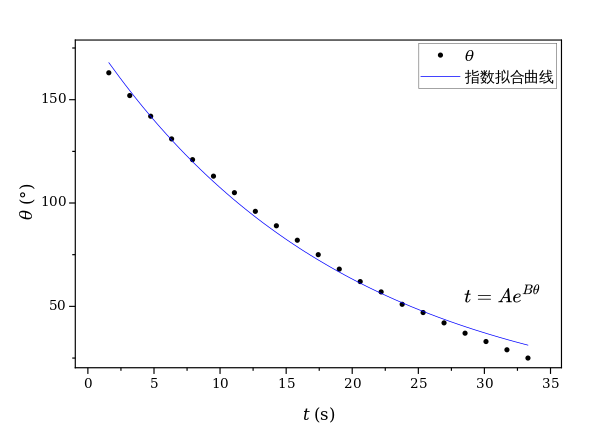
\includegraphics[scale=0.5]{exp.png}
    \caption{$\mathit{\theta}$ - $\mathit{t}$ 数据和指数拟合曲线}
    \label{fig:exp}
\end{figure}

根据 Origin Pro 的数据处理功能,得到 $\beta=0.053\pm0.001\text{ s}^{-1}$,$\omega_0$ 的平均值为 $3.963\text{ rad/s}$.

$\omega_0$ 的不确定度由周期平均值 $\bar{T_d}$ 的不确定度决定,而 $\bar{T_d}$ 的不确定度来源于取平均值和测量误差两部分:

\begin{equation}
    \sigma_{\bar{T}} = \sqrt{\frac{\sum_{i=1}^{N}(T_i-\bar{T})^2}{N(N-1)}} = 3\times10^{-4}\text{ s}
\end{equation}
\begin{equation}
    \sigma_T = 0.002\text{ s}
\end{equation}
\begin{equation}
    U_{\bar{T_d}} = \sqrt{\sigma_T^2+\sigma_{\bar{T}}^2} = 2\times10^{-3}\text{ s}
\end{equation}
\begin{equation}
    U_{\omega_0} = \sqrt{\left(\frac{\partial \omega_0}{\partial T_d}U_{T_d}\right)^2} = \frac{2\pi}{\bar{T_d}^2}U_{\bar{T_d}} = 5\times10^{-3}\text{ rad/s}
\end{equation}
\newline
由此可以计算出 $Q=\omega_0/(2\beta)=37.4$,$Q$ 的不确定度为:

\begin{equation}
    U_Q = \sqrt{\left(\frac{\partial Q}{\partial \beta}U_\beta\right)^2+\left(\frac{\partial Q}{\partial \omega_0}U_{\omega_0}\right)^2} = 0.7
\end{equation}

也就是 $Q=37.4\pm0.7$.

对于另外两种阻尼情况,重复上述步骤,得到如下数据:

% Table generated by Excel2LaTeX from sheet 'Sheet1'
\begin{longtable}{|c|c|c|c|c|c|c|}
  \caption{更高阻尼情况下振动数据} \\
    \hline
       & \multicolumn{3}{c|}{$s = 20\text{ mm}$} & \multicolumn{3}{c|}{$s = \max$} \\ \cline{1-7}
    \hline
    序号 & 振幅 $\theta_i$ ($\degree$) & 周期 $T_d$ ($\text{s}$) & 时间 ($\text{s}$) & 振幅 $\theta_i$ ($\degree$) & 周期 $T_d$ ($\text{s}$) & 时间 ($\text{s}$) \\
    \hline
    1     & 147   & 1.5842 & 1.5842 & 153   & 1.5844 & 1.5844 \\
    \hline
    2     & 123   & 1.5853 & 3.1695 & 117   & 1.5869 & 3.1713 \\
    \hline
    3     & 103   & 1.5862 & 4.7557 & 89    & 1.5883 & 4.7596 \\
    \hline
    4     & 86    & 1.5867 & 6.3424 & 68    & 1.5891 & 6.3487 \\
    \hline
    5     & 72    & 1.587 & 7.9294 & 52    & 1.5898 & 7.9385 \\
    \hline
    6     & 60    & 1.5879 & 9.5173 & 39    & 1.5901 & 9.5286 \\
    \hline
    7     & 50    & 1.5874 & 11.1047 & 29    & 1.5901 & 11.1187 \\
    \hline
    8     & 42    & 1.5872 & 12.6919 & 23    & 1.5904 & 12.7091 \\
    \hline
    9     & 35    & 1.5871 & 14.279 & 18    & 1.5908 & 14.2999 \\
    \hline
    10    & 29    & 1.5869 & 15.8659 &       &       &  \\
    \hline
    11    & 24    & 1.5868 & 17.4527 &       &       &  \\
    \hline
    12    & 20    & 1.5866 & 19.0393 &       &       &  \\
    \hline
\end{longtable}

将数据导入 Origin Pro 软件,作出散点图像,用同一公式 (Exp2PMod1) 拟合,如图 2 所示:

\begin{figure}[h]
    \begin{subfigure}[b]{0.45\textwidth}
        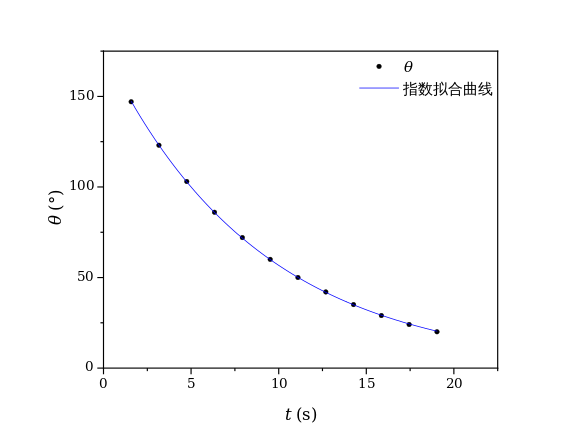
\includegraphics[scale=0.4]{exp2.png}
        \caption{$s=20\text{ mm}$}
        \label{fig:side:a}
    \end{subfigure}
    \begin{subfigure}[b]{0.45\textwidth}
        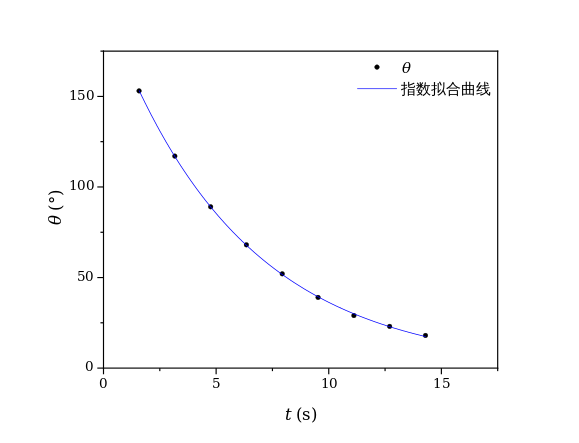
\includegraphics[scale=0.4]{exp3.png}
        \caption{$s=\max$}
        \label{fig:side:b}
    \end{subfigure}
    \caption{不同阻尼情况下的振动数据和拟合曲线}
\end{figure}

Origin Pro 给出这两种阻尼情况下的 $\beta$ 值,分别为:$s=20\text{ mm}$ 时 $\beta=0.1133\pm2\times10^{-4}\text{ s}^{-1}$;$s=\max$ 时 $\beta=0.1711\pm8\times10^{-4}\text{ s}^{-1}$. 计算得到两种情况的 $Q$,分别为:$s=20\text{ mm}$ 时 $Q=17.5$;$s=\max$ 时 $Q=11.6$.

\newpage

\subsection{受迫振动}

% Table generated by Excel2LaTeX from sheet 'Sheet1'
\begin{longtable}{|c|c|c|c|c|c|c|c|c|}
  \caption{受迫振动数据} \\
    \hline
    \multicolumn{4}{|c|}{s = 20 mm} & \multicolumn{4}{c|}{s = max} \\ \cline{1-9}
    \hline
    周期 $T$ ($\text{s}$) & 振幅 $\theta_i$ ($\degree$) & 相差 ($\degree$) & 频率 ($\text{rad/s}$) & 周期 $T$ ($\text{s}$) & 振幅 $\theta_i$ ($\degree$) & 相差 ($\degree$) & 频率 ($\text{rad/s}$) \\
    \hline
    1.6491 & 51    & 34    & 3.81006 & 1.5896 & 49    & 90    & 3.95268 \\
    \hline
    1.5853 & 80    & 90    & 3.96340 & 1.5773 & 48    & 100   & 3.98350 \\
    \hline
    1.5932 & 79    & 80    & 3.94375 & 1.5643 & 46    & 110   & 4.01661 \\
    \hline
    1.6018 & 77    & 70    & 3.92257 & 1.5505 & 42    & 120   & 4.05236 \\
    \hline
    1.6113 & 72    & 60    & 3.89945 & 1.5346 & 38    & 130   & 4.09434 \\
    \hline
    1.6229 & 65    & 50    & 3.87157 & 1.5171 & 33    & 140   & 4.14157 \\
    \hline
    1.6373 & 57    & 40    & 3.83752 & 1.4919 & 27    & 150   & 4.21153 \\
    \hline
    1.5765 & 77    & 100   & 3.98552 & 1.6026 & 48    & 80    & 3.92061 \\
    \hline
    1.5672 & 73    & 110   & 4.00917 & 1.6161 & 46    & 70    & 3.88786 \\
    \hline
    1.5577 & 67    & 119   & 4.03362 & 1.6322 & 42    & 60    & 3.84951 \\
    \hline
    1.5442 & 58    & 130   & 4.06889 & 1.6511 & 38    & 51    & 3.80545 \\
    \hline
    1.52514 & 47    & 140   & 4.11974 & 1.5953 & 49    & 85    & 3.93856 \\
    \hline
    1.4941 & 32    & 149   & 4.20533 & 1.5831 & 49    & 95    & 3.96891 \\
    \hline
    1.5837 & 81    & 91    & 3.96740 & 1.5882 & 49    & 91    & 3.95616 \\
    \hline
    1.5851 & 81    & 89    & 3.96390 & 1.5903 & 49    & 89    & 3.95094 \\
    \hline
           &       &       &       & 1.5924 & 49    & 88    & 3.94573 \\
    \hline
           &       &       &       & 1.5867 & 49    & 92    & 3.95990 \\
    \hline
           &       &       &       & 1.5224 & 34    & 137   & 4.12715 \\
    \hline
           &       &       &       & 1.5264 & 35    & 135   & 4.11634 \\
    \hline
\end{longtable}

将数据导入 Origin Pro 软件,作出幅频 ($\theta$ - $\omega$) 和相频 ($\varphi$ - $\omega$) 的散点图像,如图 3 所示:

\begin{figure}[h]
    \begin{subfigure}[b]{0.45\textwidth}
        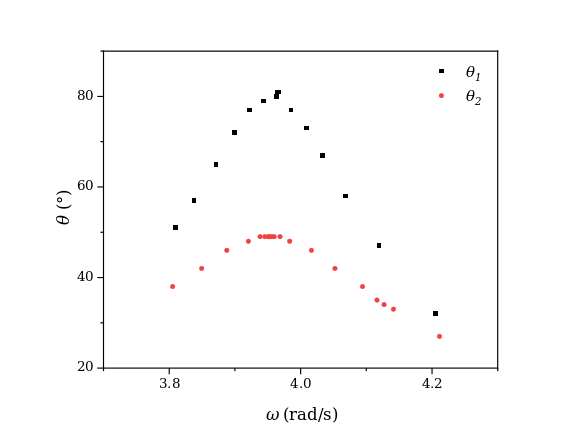
\includegraphics[scale=0.4]{fupin.png}
        \caption{\(\mathit{\theta}\) - \(\mathit{\omega}\)}
        \label{fig:side:a}
    \end{subfigure}
    \begin{subfigure}[b]{0.45\textwidth}
        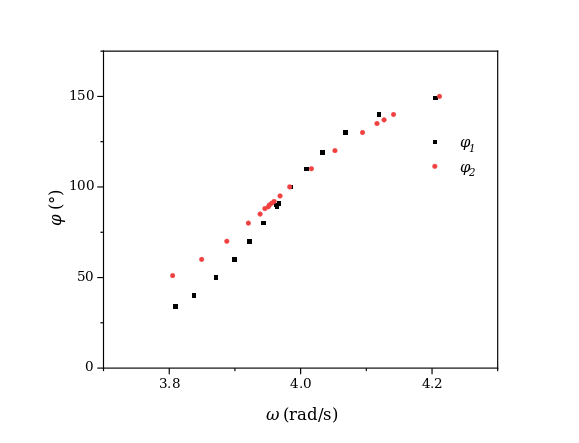
\includegraphics[scale=0.4]{xiangpin.png}
        \caption{\(\mathit{\varphi}\) - \(\mathit{\omega}\)}
        \label{fig:side:b}
    \end{subfigure}
    \caption{幅频 / 相频曲线}
\end{figure}

其中标号为 1 的是 $s=20\text{ mm}$ 的数据,标号为 2 的是 $s=\max$ 的数据.

通过观察两条曲线,得到:

1. 对于 $s=20\text{ mm}$,$\omega_r=3.966\text{ rad/s}$,$\omega_+=4.069\text{ rad/s}$,$\omega_-=3.838\text{ rad/s}$;

2. 对于 $s=\max$,$\omega_r=3.953\text{ rad/s}$,$\omega_+=4.122\text{ rad/s}$,$\omega_-=3.806\text{ rad/s}$.

因此两种情况的 $Q$ 值分别为 $17.1$ 和 $12.5$,与之前的结果较好符合.

\subsection{瞬态过程}

调整仪器,使得阻尼为 $s=20\text{ mm}$ 的情况,将电机调到共振状态,关闭电机,调整到平衡位置,之后突然开启电机,记录振幅随时间的变化,得到数据:

% Table generated by Excel2LaTeX from sheet 'Sheet1'
\begin{longtable}{|c|c|c|c|c|c|}
  \caption{瞬态过程数据} \\
    \hline
    序号    & 振幅测量值 $\theta_i$ ($\degree$) & 周期 ($\text{s}$) & 时间 ($\text{s}$) & 真实时间 ($\text{s}$) & 理论值 ($\text{rad}$) \\
    \hline
    0     & 13    & 1.6734 & 1.6734 & 1.5441 & 13.00034547 \\
    \hline
    1     & 24    & 1.6038 & 3.2772 & 3.1479 & 24.29898654 \\
    \hline
    2     & 33    & 1.5937 & 4.8709 & 4.7416 & 33.66614099 \\
    \hline
    3     & 41    & 1.5902 & 6.4611 & 6.3318 & 41.47014478 \\
    \hline
    4     & 47    & 1.5886 & 8.0497 & 7.9204 & 47.9815058 \\
    \hline
    5     & 53    & 1.5876 & 9.6373 & 9.508 & 53.41718994 \\
    \hline
    6     & 57    & 1.587 & 11.2243 & 11.095 & 57.95645574 \\
    \hline
    7     & 61    & 1.5865 & 12.8108 & 12.6815 & 61.74761008 \\
    \hline
    8     & 64    & 1.5861 & 14.3969 & 14.2676 & 64.91430971 \\
    \hline
    9     & 67    & 1.5859 & 15.9828 & 15.8535 & 67.5598351 \\
    \hline
    10    & 69    & 1.5857 & 17.5685 & 17.4392 & 69.77001094 \\
    \hline
    11    & 71    & 1.5855 & 19.154 & 19.0247 & 71.61652048 \\
    \hline
    12    & 73    & 1.5854 & 20.7394 & 20.6101 & 73.15932581 \\
    \hline
    13    & 74    & 1.5853 & 22.3247 & 22.1954 & 74.44839319 \\
    \hline
    14    & 75    & 1.5852 & 23.9099 & 23.7806 & 75.52546591 \\
    \hline
    15    & 76    & 1.5852 & 25.4951 & 25.3658 & 76.42546976 \\
    \hline
    16    & 77    & 1.5851 & 27.0802 & 26.9509 & 77.17747123 \\
    \hline
    17    & 77    & 1.585 & 28.6652 & 28.5359 & 77.80581591 \\
    \hline
    18    & 78    & 1.585 & 30.2502 & 30.1209 & 78.33087372 \\
    \hline
    19    & 78    & 1.5849 & 31.8351 & 31.7058 & 78.76959761 \\
    \hline
    20    & 79    & 1.585 & 33.4201 & 33.2908 & 79.13622963 \\
    \hline
    21    & 79    & 1.5849 & 35.005 & 34.8757 & 79.44257729 \\
    \hline
    22    & 80    & 1.5849 & 36.5899 & 36.4606 & 79.69857063 \\
    \hline
\end{longtable}

因为实验开始时仪器还未正常开始测量,所以要对时间数据进行修正,真实时间并不是周期数据的简单叠加,而是要使用之前已经得到的阻尼系数 $\beta$ 解出最开始的时间. 利用第一组数据,在振幅为 $13\degree$ 时,有如下方程:

\begin{equation}
    13\degree = \theta_{\max}(1-e^{-\beta t}) = 81\degree(1-e^{-\beta t})
\end{equation}

解得真实时间 $t=1.5441\text{ s}$,所以对剩下的时间数据都做一个平移,得到真实时间数据. 将数据导入 Origin Pro 软件,作出振幅随时间变化的散点图,同时将理论值 $\theta_i=\theta_{\max}(1-e^{-\beta t})$ 画在同一张图中,如图 4 所示:

\begin{figure}[h]
    \centering
    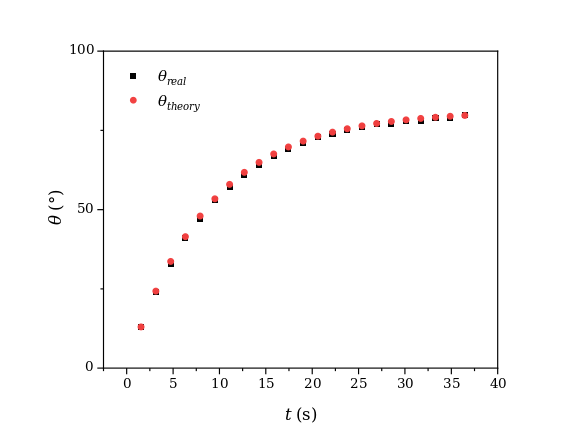
\includegraphics[scale=0.5]{shuntai.png}
    \caption{瞬态过程数据和理论曲线}
    \label{fig:shuntai}
\end{figure}

可以看出,理论与实验符合得相当好.

\section{分析与讨论}

\subsection{课堂习题}

(A.0) 说明 $\beta$ 的单位 (量纲) 是什么?

显然 $\dim{\beta}=\text{T}^{-1}$,单位是 $\text{s}^{-1}$.

(B.1) 证明欠阻尼下幅频和相频的共振频率近似相等.

两种曲线的共振频率分别为 $\omega_\theta=\sqrt{\omega_0^2-\beta^2}$ 和 $\omega_\varphi=\omega_0$,在欠阻尼情况下 $\beta\ll\omega_0$,所以 $\omega_\theta\approx\omega_\varphi$,近似相等.

(B.2) 如何判断受迫振动达到稳态?

当仪器上显示的驱动力周期和振动周期相等时,受迫振动达到稳态.

(C.3) 振动系统达到稳态时,求电机在一个周期内提供的平均输入功率的表达式 (用 $\theta_m$,$\omega_0$,$k$ 和 $Q$ 表示).

在稳态时,振动系统的能量不再随时间变化,所以输入功率等于阻尼力的功率. 阻尼力功率为 $P_d=2k\beta\theta_m^2\sin^2(\omega_0t-\varphi)$ ($k$ 为弹簧劲度),故平均功率为:

\begin{equation}
    P_{\text{in}} = \frac{1}{T}\int_0^TP_d\text{d}t = k\beta\theta_m^2
\end{equation}

\subsection{不足之处和改进方案}

在我的实验中有一些不足之处:\newline

1. 用 Origin 做数据的拟合时,并未考虑将 $\sigma_T=0.002\text{ s}$ 的这部分不确定度考虑进 $\beta$ 的不确定度中,这会造成一个不可忽视的影响,因为本身 Origin 给出的不确定度就是 $10^{-3}\text{ s}$ 量级.

下面我们尝试进行估计:

\begin{equation}
    U_{\beta} = \sqrt{\left(\frac{\partial \beta}{\partial T_d}U_{T_d}\right)^2+0.001^2} = 0.005\text{ s}^{-1}
\end{equation}
\newline
这样就能得到更加准确的 $\beta$ 的不确定度.\newline

2. 在瞬态过程中,由于仪器的误差,我们并不能保证实验开始时的振幅就是仪器的显示值,这和最开始的周期测量不准的原因是一样的,因为第一周期开始时仪器还没有开始反应,所以理论上来说不止要对时间进行修正,还要对振幅进行修正.

我个人的建议:做一个更小的阻尼,比如把 $s=20\text{ mm}$ 改成 $s=10\text{ mm}$,等到仪器开始稳定工作之后再开始记录数据,这样既保证了实验数据的总量不小于 $15$ 组,也能够更准确的记录曲线.\newline

3. 考虑使用 python 进行幅频曲线或者相频曲线的拟合.

我们以 $s=20\text{ mm}$ 的阻尼所对应的幅频曲线为例,用 python 进行拟合,所使用的代码如下:

\begin{minted}[language=python]{python}
    from numpy import sqrt
    import numpy as np
    import matplotlib.pyplot as plt
    from scipy.optimize import curve_fit
    import matplotlib as mpl
    mpl.rcParams['font.sans-serif'] = ['LXGW WenKai']  # 解决中文不显示问题
    plt.rcParams['axes.unicode_minus'] = False       # 解决负数坐标显示问题

    # 从终端读取输入数据
    x = list(map(float, input("请输入 x 的值(用空格分隔):").split()))
    y = list(map(float, input("请输入 y 的值(用空格分隔):").split()))

    x = np.array(x)
    y = np.array(y)

    # 对 x 和 y 进行排序
    sorted_indices = np.argsort(x)[::-1]
    x = x[sorted_indices]
    y = y[sorted_indices]

    # 变量一定要放在第一个位置,定义我们要使用的函数.
    def func(x, a, b, c):
        return a*b/sqrt((a**2-x**2)**2+4*c**2*x**2)

    popt, pcov = curve_fit(func, x, y) 
    print(popt) 
    print(pcov)
    # popt[0], popt[1], popt[2] 分别代表参数 a, b, c
    y2 = func(x, popt[0], popt[1], popt[2])

    plt.scatter(x, y, marker='x', lw=1, label='原始数据')
    plt.plot(x, y2, c='r', label='拟合曲线')
    plt.legend() # 显示标签
    plt.show()
\end{minted}

将我们的数据输入,得到终端输出结果为:

\begin{minted}[language=bash]{bash}
    [ 3.96031646 18.80302683  0.11716302]
    [[1.00527387e-06 1.20679138e-05 1.10673460e-07]
     [1.20679138e-05 4.17491847e-02 2.98762905e-04]
     [1.10673460e-07 2.98762905e-04 2.28624662e-06]]
\end{minted}

同时输出图像如下:

\begin{figure}[h]
    \centering
    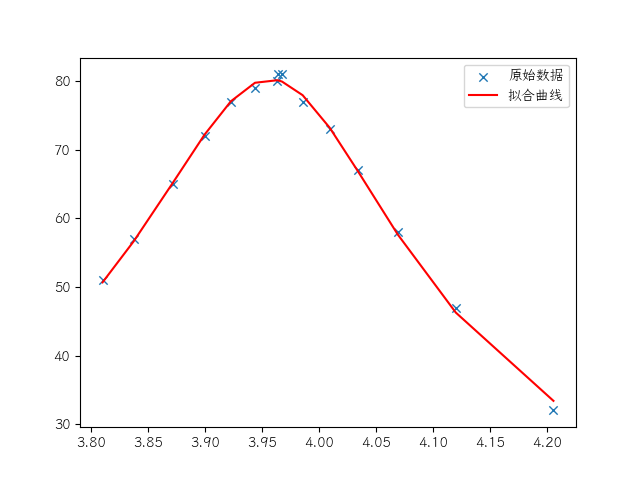
\includegraphics[scale=0.5]{python.png}
    \caption{用 python 进行拟合的结果}
    \label{fig:python}
\end{figure}

这一输出结果效果较好,推荐放到之后的课堂教学中讲解.
\newpage

\section{原始数据截图}

\begin{figure}[h]
    \centering
    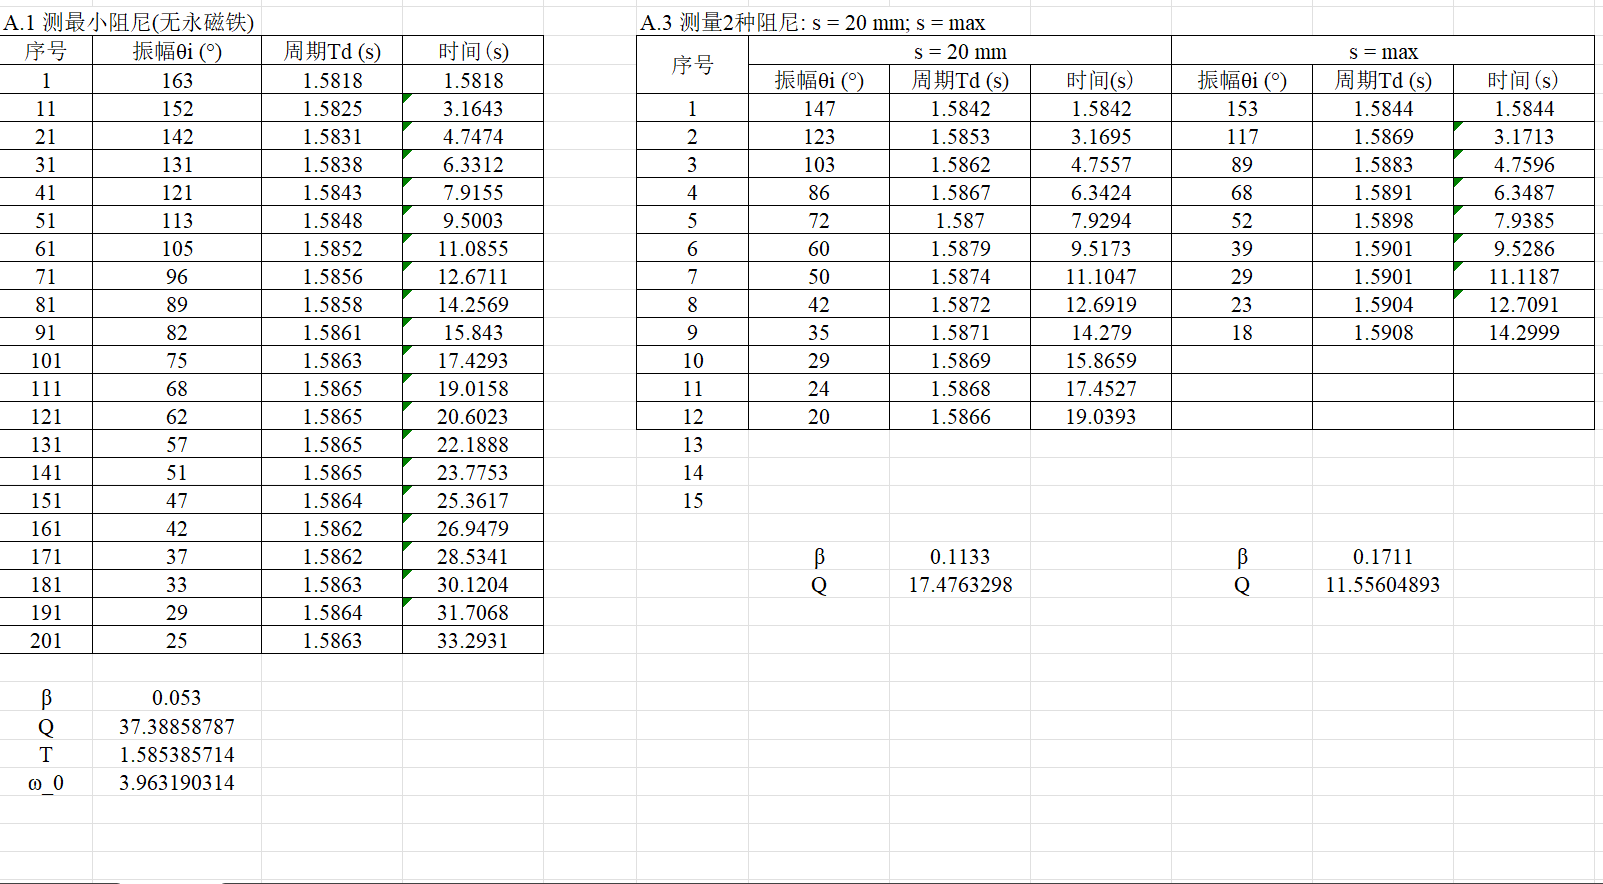
\includegraphics[scale=0.3]{yuanshishujv1.png}
    \caption{实验原始数据截图 (1)}
    \label{fig:data}
\end{figure}
\begin{figure}[h]
    \centering
    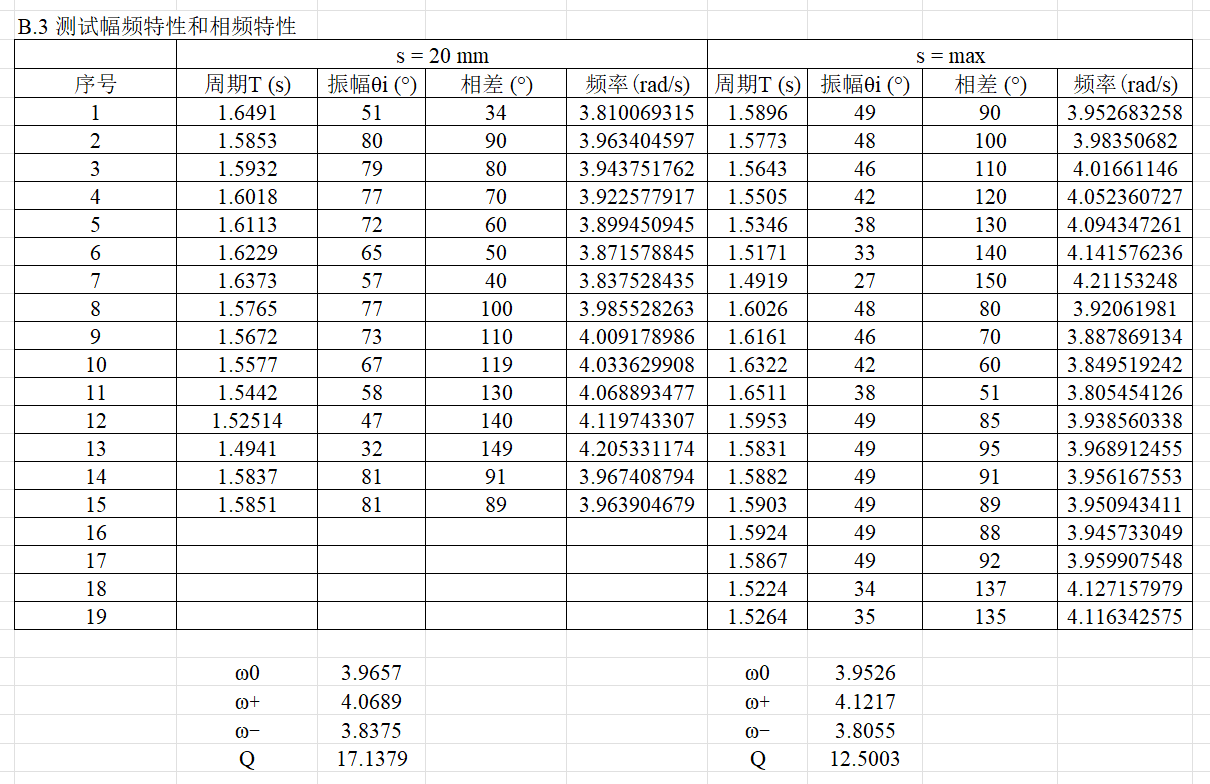
\includegraphics[scale=0.3]{yuanshishujv2.png}
    \caption{实验原始数据截图 (2)}
    \label{fig:data}
\end{figure}
\begin{figure}[h]
    \centering
    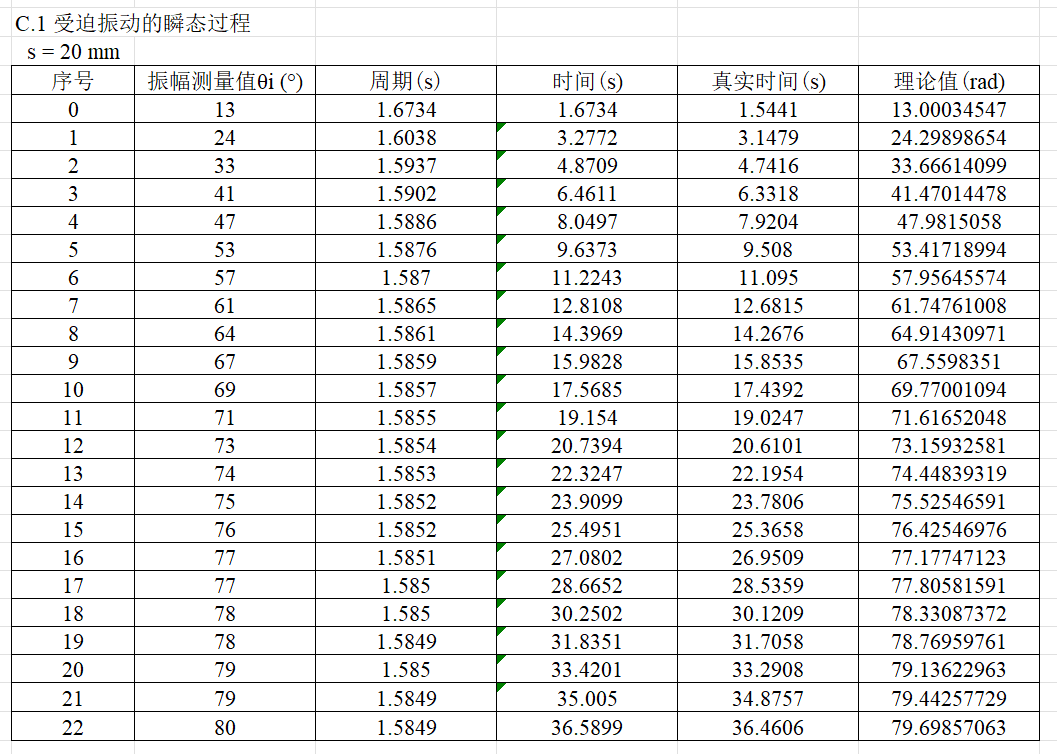
\includegraphics[scale=0.3]{yuanshishujv3.png}
    \caption{实验原始数据截图 (3)}
    \label{fig:data}
\end{figure}

\end{document}
